\documentclass[11pt,a4paper,oneside]{article}
\usepackage[dvipsnames, svgnames, x11names]{xcolor}
\usepackage{euler,amsthm,amsmath,amsfonts,graphicx,epigraph,indentfirst,enumerate,comment,listings,fontspec,color,subcaption,listings}
\usepackage{xeCJK}
\usepackage{hw}
\usepackage{pythonhighlight}
\usepackage{tikz}
\usepackage{algorithm}
\usepackage{algpseudocode}
\usepackage{float}

\newcommand{\nth}[1]{#1\textsuperscript{th}}
\newcommand{\E}{\mathop{\mathbb{E\/}}}
\newcommand{\N}{\mathbb{N}}
\newcommand{\R}{\mathbb{R}}

\renewcommand{\hwtitle} {CS217 Homework 2, First Submission}	
\renewcommand{\hwauthor}{Akina}
\renewcommand{\hwdate}{\today}

\begin{document}
\title{\hwtitle}
\author{\hwauthor}
\date{\hwdate}
\maketitle

\section*{Minimum Spanning Trees}

Throughout this assignment, let $G$ be a weighted graph, i.e., $G=(V,E,w)$ 
with $w: E \rightarrow \R^+$.
For $c \in \R$ and a weighted graph $G = (V,E,w)$, let
$G_c := (V, \{e \in E \ | \ w(e) \leq c\})$. That is, $G_c$ is the
subgraph of $G$ consisting of all edges of weight at most $c$.

\begin{problem}{1}
	\statement
	Let $T$ be a minimum spanning tree of $G$, and let $c \in \R$.  Show that
	$T_c$ and $G_c$ have exactly the same connected components.  (That
	is, two vertices $u,v \in V$ are connected in $T_c$ if and only if
	they are connected in $G_c$).
	You are encouraged to draw pictures to illustrate your proof!
	\solution
	
	\begin{proof}
		\(\Rightarrow\): \(T_c\) is a subgraph of \(T\) consisting of all edges of weight at most \(c\). SInce \(T \subseteq G\), then we have  \(T_c = T \cap G_c\). This implies that \(T_c \subseteq G_c\) if two vertices \(u, v\) are connected in \(T_c\), they are connected in \(G_c\).
		
		\(\Leftarrow\): we prove the contrapositive propostion: If two vertices \(u, v\) are not connected in \(T_c\), neither in \(G_c\). Considering Kruskal’s Algorithm
		
		\begin{enumerate}
			\item Sort edges from cheap to expensive
			\item Add to \(X\) the cheapest edge that does not create a cycle.
		\end{enumerate}
	
		Given a minimum spanning tree \(T\), there exist an avaliable order of edges(by reorder the edges with same weight) such that the comeout of Kruskal's Algorithm is exactly \(T\). When we deal with a specific edge \(e\), analyse two cases: 
		
		\begin{enumerate}
			\item \(e \in T\), \(e\) connects two components.
			\item \(e \not\in T\), \(e\) introduce a circle. i.e. \(e\) doesn't Change the connectivity of any two vertices.
		\end{enumerate}
	
		If the Algorithm Stops before processing \(e_{i+1}\), then we get \(T_c\) and \(G_c\), in which \(w(e_{i}) \leq c < w(e_{i + 1})\). If two vertices \(u, v\) are not connected in \(T_c\), neither in \(G_c\), since the other edges make no change of connectivity.
		
		Especially, If \(c\) bigger than the most expensive, \(G_c := G\), \(T_c := T\), they are all connected.
	\end{proof}
\end{problem}

\begin{problem}{2}
	\statement
	For a weighted graph $G$, let $m_c(G) := | \{ e \in E(G) \ | \ w(e) \leq c\}|$, i.e.,
	the number of edges of weight at most $c$ (so $G_c$ has $m_c(G)$ edges).
	Let $T, T'$ be two minimum spanning trees of $G$. Show that
	$m_c(T) = m_c(T')$.

	\solution
	
	We prove it by reduction to absurdity. Without loss of generality, let \(m_c(T) > m_c(T')\). There exist at least one edge, donated by \(e = \{u, v\}\), such that \(e \in T\) but \(e \not\in T'\). \(T'_c\) is a good set since it is a subgraph of a minimum spaning tree \(T'\), find a cut \(S\) of \(T'_c\) contains \(u\) but not \(v\).
	
	Analyse two cases:
	
	\begin{enumerate}
		\item if \(e \in T'\), \(w(e) \leq c\), then \(e \in T'_c\), a contradiction.
		\item if \(e \not\in T'\) and \(u, v\) not connected in \(T\), we can find a circle \(u \xrightarrow{T'} v \xrightarrow{e}\), each edge of \(u \xrightarrow{T'} v\) has weight not grea
	\end{enumerate}
	
\end{problem}
\begin{problem}{3}
	\statement
	Suppose $G$ is connected, and no two edges of $G$ have the same weight. 
	Show that $G$ has exactly one minimum spanning tree!
	
	\solution
\end{problem}

\section*{Quickselect}

A {\em multigraph} is a graph that can have multiple edges, called
``parallel edges''. Without defining 
it formally, we illustrate it:
\begin{center}
	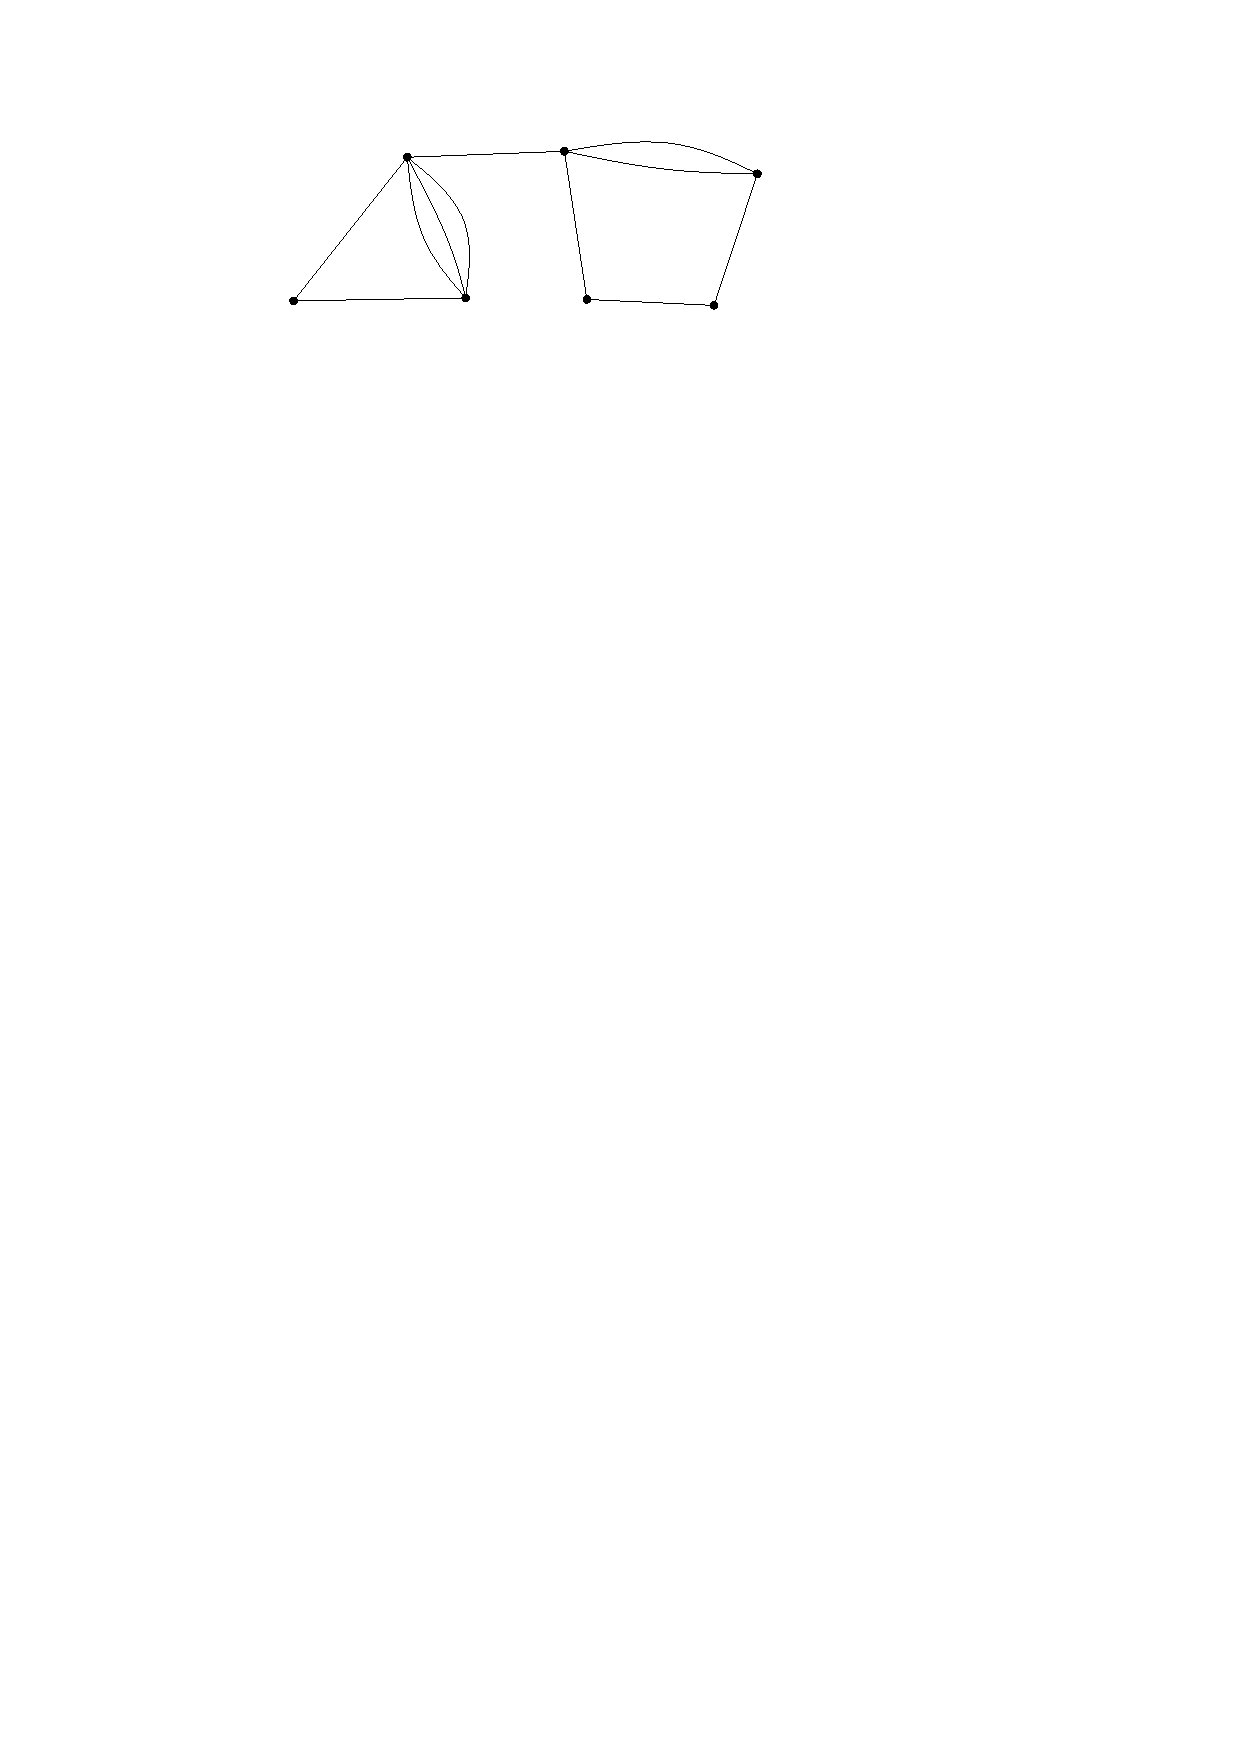
\includegraphics[width=0.6\textwidth]{figures/multigraph.pdf}\\
	A multigraph.
\end{center}
All other definitions, like connected components and spanning trees
are the same as for normal (simple) graphs. However,
when two spanning trees use different parallel edges, we consider them
different:
\begin{center}
	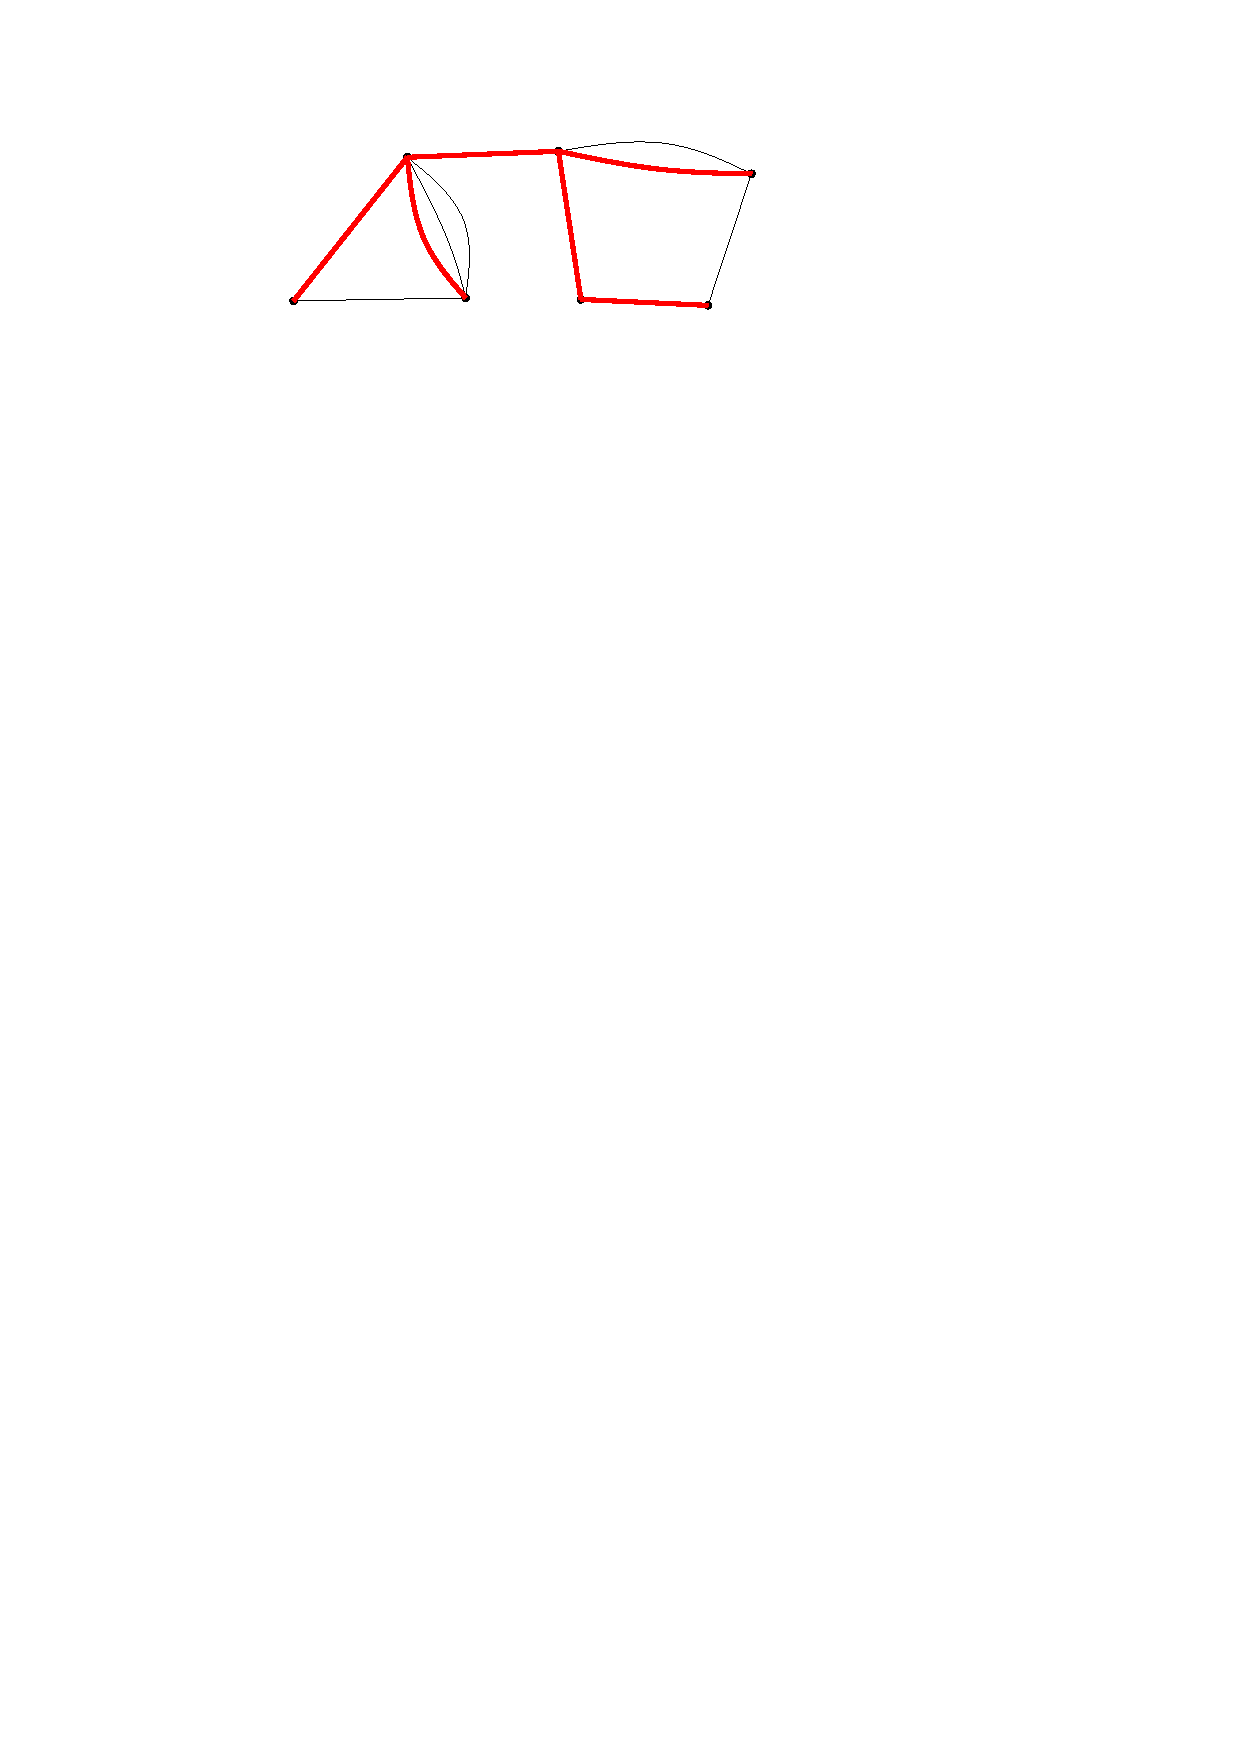
\includegraphics[width=0.4\textwidth]{figures/multigraph-forest.pdf} \hspace{2cm}
	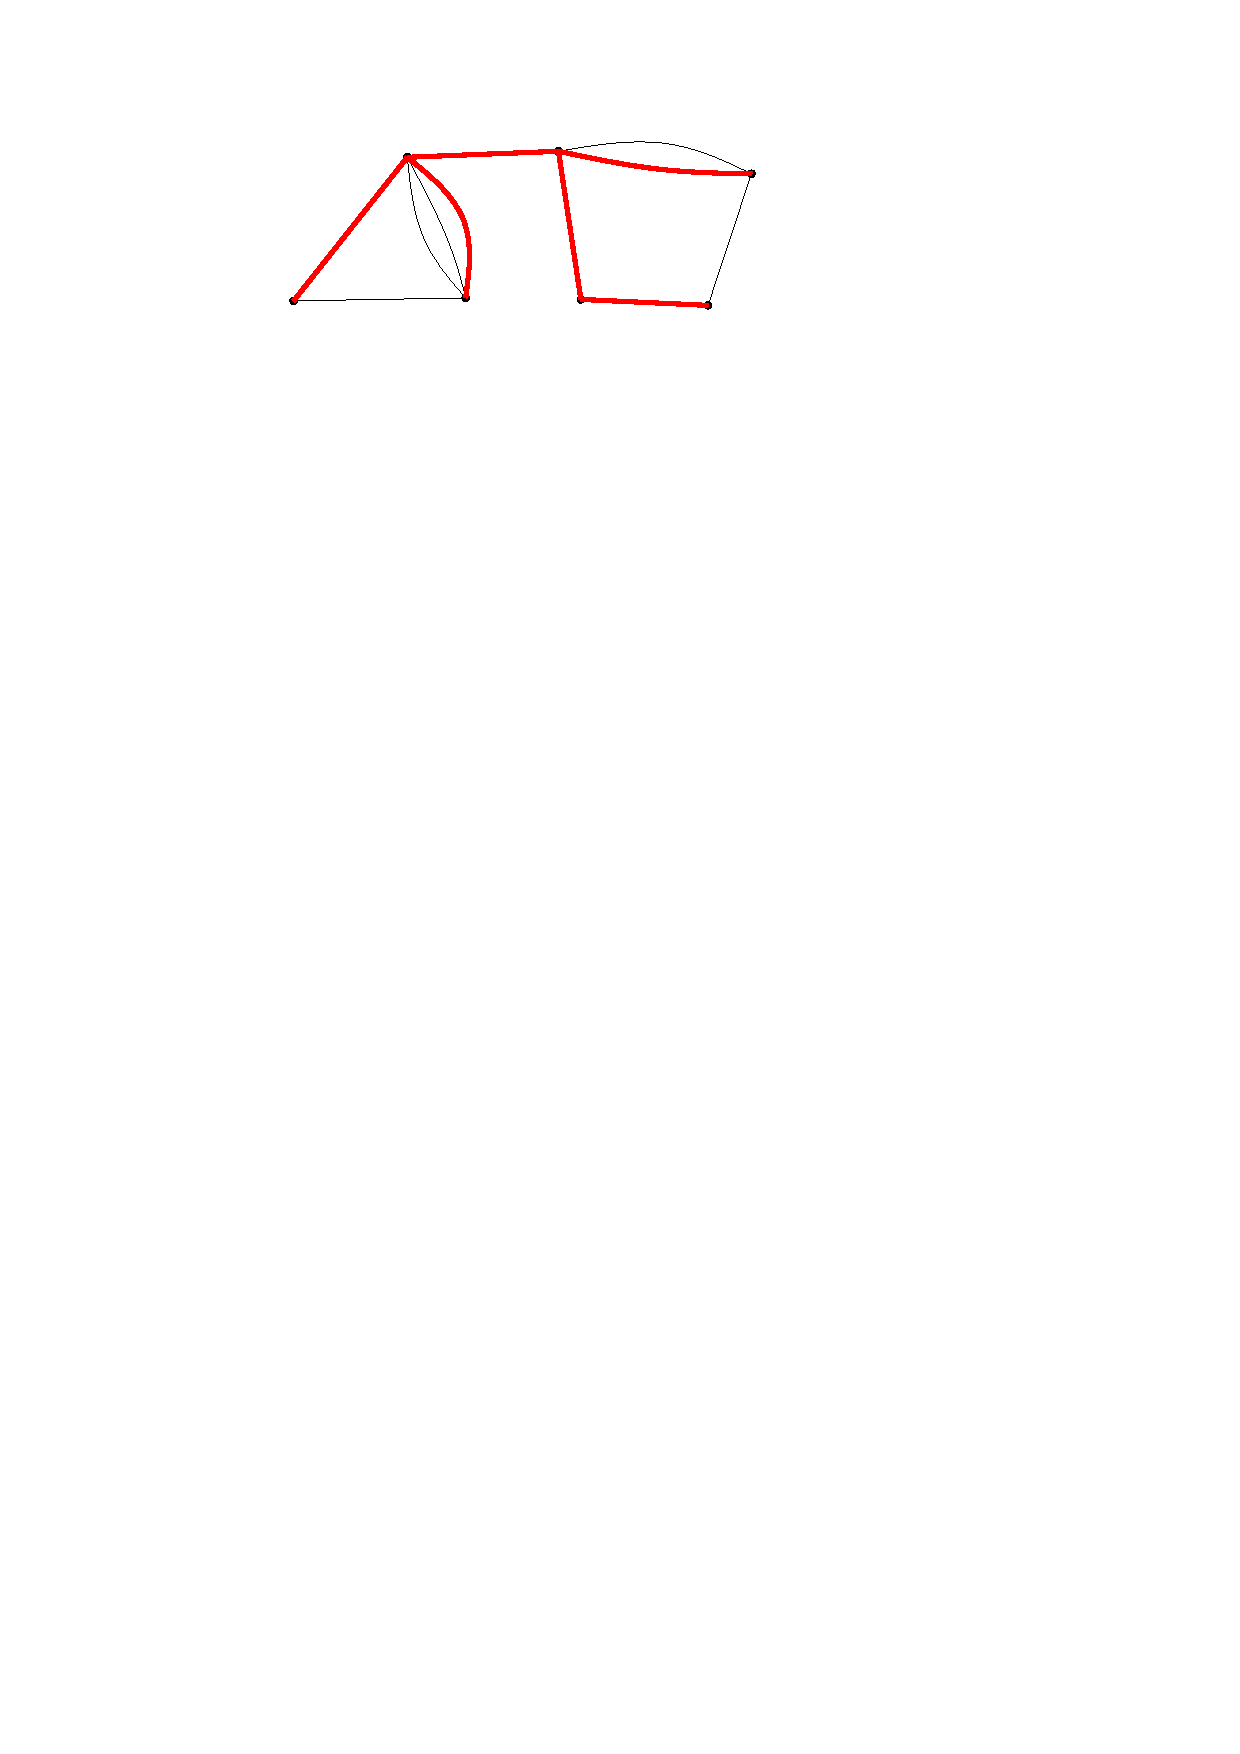
\includegraphics[width=0.4\textwidth]{figures/multigraph-forest-other.pdf} \\
	The same multigraph with two different spanning trees.
\end{center}

\begin{problem}{4}
\statement
How many spanning trees does the above multigraph on 7 vertices have?
Justify your answer!

\end{problem}

\begin{problem}{5}
\statement
Suppose you have a polynomial-time algorithm that, given a multigraph $H$,
computes the number of spanning trees of $H$.
Using this algorithm as a subroutine, design a polynomial-time algorithm
that, given a weighted graph $G$, computes the number of 
minimum spanning trees of $G$.

\solution

\end{problem}

\end{document}
